% The font can be either 10pt or 12pt to conform to UNCC standards.  Change it here if you like.
\documentclass[12pt]{article}

\usepackage{packages/thesis}
% This line makes sure that single-line captions won't automatically center. 
\usepackage{caption} % Should this move to unccspecs.sty?
\captionsetup{singlelinecheck=false}

%%%%%%%%%%%%%%% OPTIONAL PACKAGES YOU MAY WANT TO CONSIDER %%%%%%%%%%%%%%%
% Uncomment the \usepackage{} command to add the environments to your document. Note that Miktex may need to download the package the first time you add the package, so be patient, especially if you enable a lot of these packages at once.

% Add colors to your text.  Excellent tool for leaving yourself notes. (http://en.wikibooks.org/wiki/LaTeX/Colors)
%\usepackage{color}

% It supplies a landscape environment, and anything inside is basically rotated. (http://en.wikibooks.org/wiki/LaTeX/Page_Layout)
%\usepackage{lscape}

% A set of useful symbol fonts (http://www.ctan.org/pkg/ifsym)
%\usepackage{ifsym}

% supports the creation of indices, like at the end of most books (http://en.wikibooks.org/wiki/LaTeX/Indexing)
%\usepackage{makeidx}

% Allows the manipulation of graphics (http://en.wikibooks.org/wiki/LaTeX/Importing_Graphics)
%\usepackage{graphicx}

%         The package alters the command \_ (which normally prints an underscore character or facsimile) so that the hyphenation of constituent words is not affected, and hyphenation is permitted after the underscore. (http://ctan.mirrorcatalogs.com/macros/latex/contrib/underscore/underscore.pdf)
%\usepackage{underscore}

%  Everything input between the begin and end commands are processed as if by a typewriter (http://en.wikibooks.org/wiki/LaTeX/Paragraph_Formatting). Useful for adding code blocks/listings
%\usepackage{verbatim}

%  Used with verbatim to include the source code of any programming language within your document
%\usepackage{listings}

% Helps format tables using the \toprule, \midrule, and \bottomrule commands (http://en.wikibooks.org/wiki/LaTeX/Tables#Using_booktabs)
%\usepackage{booktabs}

%  Helps format tables (http://en.wikibooks.org/wiki/LaTeX/Tables#Using_array)
%\usepackage{array}

% Allows columns spanning multiple rows in the table environment (http://en.wikibooks.org/wiki/LaTeX/Tables)
%\usepackage{multirow}

% Allows rotating of any object (http://en.wikibooks.org/wiki/LaTeX/Rotations)
%\usepackage{rotating}

% Allows captions in figures and tables. Especially useful when used with subcaptions if doing subfigures (http://en.wikibooks.org/wiki/LaTeX/Floats,_Figures_and_Captions)
%\usepackage{caption}

% Will arrange the figures or tables side-by-side (http://en.wikibooks.org/wiki/LaTeX/Floats,_Figures_and_Captions)
%\usepackage{subcaption}

% Balances columns on the last page. Not very useful here, but very useful in scholarly papers to balance your last page (http://www.ctan.org/pkg/flushend)
%\usepackage{flushend}

% Inserts hypertext markups into document (so digital copies have a table of contents which links to chapters, sections, figures, etc.) (https://www.tug.org/applications/hyperref/manual.html)
%\usepackage[pdftex]{hyperref}

% Creates a compact list (http://www.howtotex.com/packages/compact-lists-with-paralist/)
%\usepackage{paralist}
%%%%%%%%%%%%%%%%%%%%%%%%%%%%%%%%%%%%%%%%%%%%%%%%%%%%%%%%%%%%%%%%%%%%%%%%%%%%%%%


% This line decides how deep the Table of Contents will go.  
% A tocdepth of 1 means it will only show chapters and sections.
% You can increase it if you want your Table of Contents to show 
% subsections (tocdepth = 2) or subsubsections (tocdepth = 3) as well.
\setcounter{tocdepth}{2}

\begin{document}

% !!!!!!!!!!!! WARNING !!!!!!!!!!!!!!
%
% When printing your thesis, pay attention to the "Page Scaling" option on the print setup page!
% DO NOT choose the option "Fit to Printable Area."
% This is the default option in Adobe and it will make your formatting wrong!
%  Make sure you change this option to "None."
%
% !!!!!!!!!!!!!!!!!!!!!!!!!!!!!!!!!!!!!!!!

\startprelim

\author{UNCC PhD Student}
\title{Quantifying the Unquantifiable}

% Doctype should be either dissertation proposal, dissertation, or thesis.
% If you're getting a master's, use "thesis."  If you're getting a PhD, use "dissertation."

\doctype{dissertation}

% These should be self-explanatory.

\degree{Doctor of Philosophy}
\major{Computing and Information Systems}
\publicationyear{2013}

\advisor{Dr. My Advisor}

% Add the full name and title of all your committee members, 
% apart from your advisor, one by one.  The style file expects
% 3 to 5 committee members in addition to your advisor.

\committeeMember{Dr. Committee Member 1}
\committeeMember{Dr. Committee Member 2}
\committeeMember{Dr. Committee Member 3}
\committeeMember{Dr. Committee Member 4}

% Generate the preliminary pages (title page, copyright page, 
% abstract page, and table of contents) in the following order.

\maketitlepage

\makecopyright

\abstract{
In this dissertation, I convince you that I should be allowed to graduate. 
}

\acknowledgments{
We would like to thank ..............
:) :) :)
}

\listofcontentsfigurestables

\startbody

% Write chapter titles in ALL CAPS.
% Write \bodysection & \bodysubsection in normal title caps
% Sections can be labeled \label{Introduction}

\bodychapter{INTRODUCTION}
\label{Intro}

There is a substantial body of work in HCI that guides the evaluation of productivity support tools. Shneiderman compared the growing community of researchers developing and studying creativity support tools to the earlier rise of researchers working on productivity support tools~\cite{Shneiderman:2007wp}. He said that researchers in CSTs are ``moving from the comparatively safe territory of productivity support tools to the more risky frontier of creativity support tools.'' Shneiderman noted that one of the challenges that makes CST research `risky' is that there are no obvious measures of success~\cite{Shneiderman:2007wp}. 

\begin{table}[t]
\centering
\scriptsize
\caption[Overview of Creativity Support Tools]{A summary of creativity support tools, including examples from research and industry.}
\begin{tabular}{|l|l|}
\hline
\textbf{Category} & \textbf{Example} \\
\hline
Visualization \& Simulation  & Tableau, D3, netLogo \\
Concept Mapping \& Information Collage & combinFormation, Visio, Omnigraffle \\
Architectural \& Design & AutoCAD, Rhino3D \\ 
Mathematics & SPSS, MatLab, WolframAlpha \\
Software development environments & Eclipse, Visual Studio \\
Video Editing & Final Cut Pro, iMovie \\
Drawing/Painting &  Illustrator, InkScape, CorelDraw \\
Animation & Flash, Maya, SoftImage, Houdini \\
Music & GarageBand, Zya, Sequel, NodeBeat \\
Photography & Photoshop, Lightroom \\
Wikis, Blogs, \& Online Presence  & MediaWiki, WordPress, DreamWeaver \\
Writing \& Presentation & Google Docs, MS Word, Prezi \\
\hline
\end{tabular}
\label{CSTSummary}
\end{table}%

\begin{figure}[t]
\centering
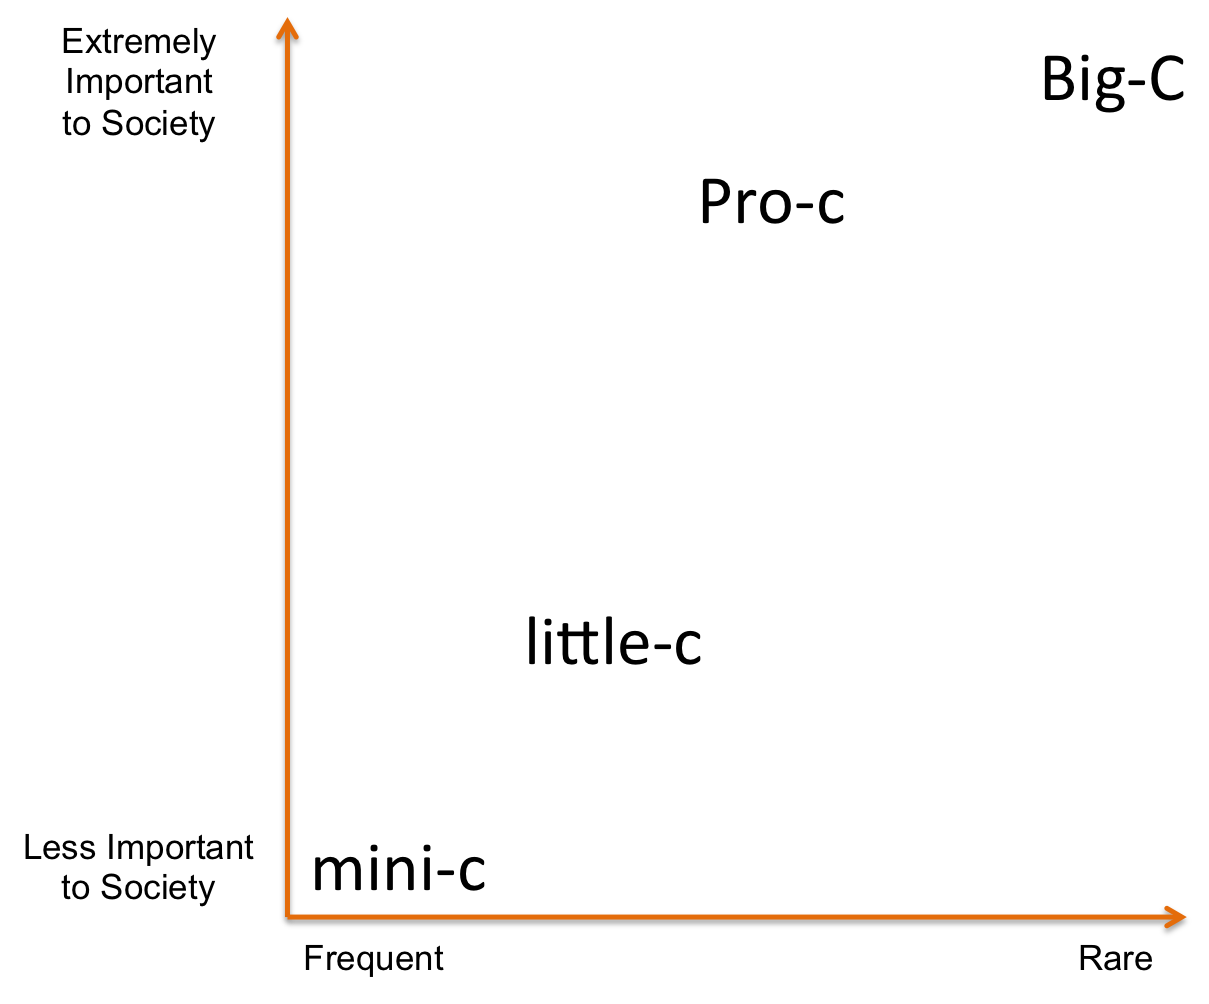
\includegraphics[width=4in]{images/spectrum.png}
\caption[Novelty-Impact Space of Creativity]{The creativity literature contains classifications of creative contributions across two dimensions: the Novelty-Impact space. Highly novel contributions are more rare, contributions with minimal novelty are more frequent.}
\label{NIspace}
\end{figure}

\begin{figure}[t]
\centering
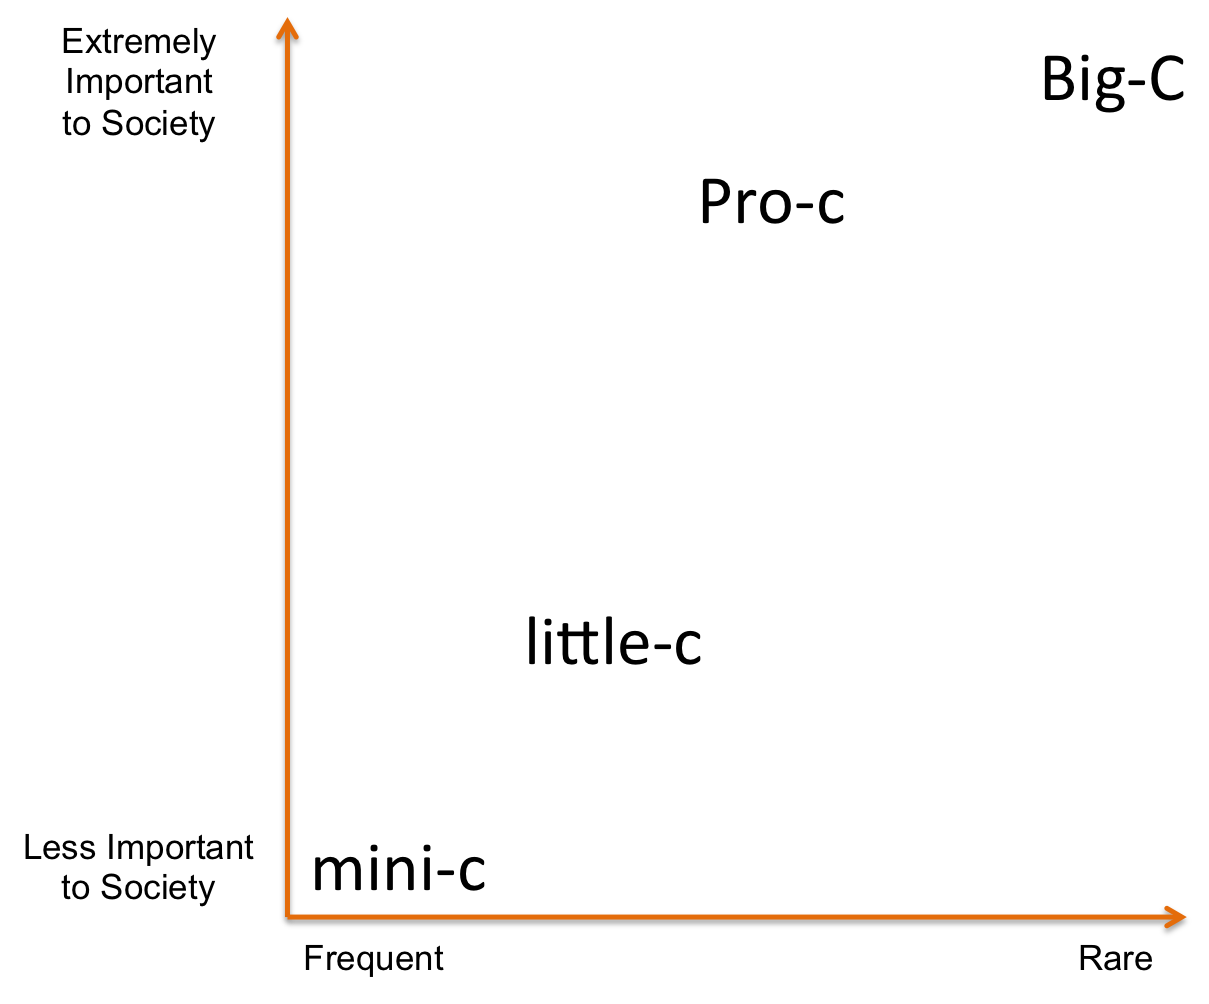
\includegraphics[width=4in]{images/spectrum.png}
\caption{The creativity literature contains classifications of creative contributions across two dimensions: the Novelty-Impact space. Highly novel contributions are more rare, contributions with minimal novelty are more frequent.}
\end{figure}

\bodysection{I have a super super super super super super super super super super super long title}
\bodysubsection{Another super super super super super super super super super super super super super super long title}

\bodysubsection{Evaluation of Creativity Support Tools}
\label{CSTEvaluation}
While there is an extensive history of evaluating creativity, the evaluation of tools to support creativity is a much newer field of study. As previously discussed, Shneiderman noted that the evaluation of creativity support tools is challenging because there are no obvious metrics for researchers to quantify~\cite{Shneiderman:2007wp}. 



\clearpage 

\startbib

\bibliography{dissertation}

\finishbib
\clearpage 

\appendix
%\addtocontents{toc}{\parindent0pt\vskip12pt APPENDICES\par} %toc entry, no page #


\appendixchapter{APPENDIX A: MEAN VALUES IN THE FIRST VISUALIZATION EXPERIMENT}
This is the first appendix
\clearpage 

\appendixchapter{APPENDIX B: MEAN VALUES IN THE SECOND VISUALIZATION EXPERIMENT}
This is the second appendix

\clearpage 


%\begin{publications}
%  \pubitem{Yi Shen, Publication1}
%  \pubitem{Yi Shen, Publication2}
%\end{publications}
\end{document}
